\PassOptionsToClass{fontset=fandol}{ctexart}
\documentclass{rjthesis}
\usepackage{booktabs}
\usepackage{amsmath}
\usepackage{graphicx}
\usepackage{array}
\usepackage{float}
\usepackage{makecell}
\usepackage[backend=biber,style=numeric,sorting=none,giveninits=true,defernumbers=true]{biblatex}
\addbibresource{references.bib}

\defbibheading{rjrefs}{\section*{#1}}
\defbibheading{rjcnrefs}{%
	\par\vspace{8pt}
	{\xiaowuhao\noindent \textbf{#1}\par}
}
\AtBeginBibliography{\rjbibfont}
\setlength{\bibitemsep}{0pt}

\rjhead{作者 等:面向动态交通场景的静态-动态解耦多模态路径表示学习方法}

\rjtitle{面向动态交通场景的静态-动态解耦多模态路径表示学习方法\textsuperscript{*}}
\rjauthor{高宇岑\textsuperscript{1}, 王雪凝\textsuperscript{2}, 庄新鱼\textsuperscript{2}, 王斌\textsuperscript{2}, 杨晓春\textsuperscript{1}}
\rjinfor{\textsuperscript{1}(东北大学软件学院, 沈阳, 110169)\\
\textsuperscript{2}(东北大学计算机学院, 沈阳, 110169)\\
通讯作者: 杨晓春, E-mail: yangxc@mail.neu.edu.cn
}
\rjabstracttext{准确的路径表示是旅行时间估计、路径排序和轨迹分析等智能交通任务的基础.现有路径表示学习方法通常依赖路网拓扑、道路属性或道路文本语义等相对静态的信息,难以刻画同一路径在不同时刻受交通状态变化影响而产生的动态差异.针对这一问题,本文提出一种面向动态交通场景的静态-动态解耦多模态路径表示学习方法DynaPath-Lite.该方法将路径数据组织为静态模态$\mathbf{X}^{sta}=\{\mathbf{X}^{topo},\mathbf{X}^{sem}\}$和动态模态$\mathbf{X}^{dyn}_{\tau}$:静态模态描述路网拓扑、道路属性和道路文本语义,可离线编码并缓存;动态模态描述近期速度、旅行时间、拥堵状态和观测密度,随历史轨迹在线增量更新.在此基础上,本文设计层次化跨模态对齐机制,先在道路级对齐拓扑与语义表示,再在路径级对齐静态路径表示与指定时刻的动态状态表示;同时提出可靠性感知动态融合方法,根据观测数量、缺失率和数据时效性调节动态模态权重,使模型在动态数据充分时更信任实时状态,在观测稀疏或缺失时自动退化为静态表示.本文在真实出租车轨迹数据集上进行旅行时间估计实验,并采用时间顺序切分和历史窗口增量构建动态特征以避免未来信息泄漏.实验结果表明,动态增强模型相较静态梯度提升基线将MAE由88.60秒降低至85.22秒,相对提升3.8\%;在线性模型中,动态特征也带来约5.8\%的MAE改进.结果说明,面向不同更新频率和不同可靠程度的多模态路径数据进行解耦组织、分层对齐和可靠性融合,能够有效提升动态交通场景下的路径表示质量.}
\rjkeywords{多模态数据融合; 路径表示学习; 动态交通状态; 旅行时间估计; 轨迹数据管理; 大语言模型}
\rjclc{TP391}
\rjcncite{高宇岑,王雪凝,庄新鱼,王斌,杨晓春.面向动态交通场景的静态-动态解耦多模态路径表示学习方法.软件学报,20XX,XX(XX):1--XX. http://www.jos.org.cn/1000-9825/0000.htm}
\rjencite{Gao YC, Wang XN, Zhuang XY, Wang B, Yang XC. Static-dynamic decoupled multimodal path representation learning for dynamic traffic scenarios. Ruan Jian Xue Bao/Journal of Software, 20XX,XX(XX):1--XX (in Chinese). http://www.jos.org.cn/1000-9825/0000.htm}
\rjetitle{Static-Dynamic Decoupled Multimodal Path Representation Learning for Dynamic Traffic Scenarios}
\rjeauthor{GAO Yu-Cen\textsuperscript{1}, WANG Xue-Ning\textsuperscript{2}, ZHUANG Xin-Yu\textsuperscript{2}, WANG Bin\textsuperscript{2}, YANG Xiao-Chun\textsuperscript{1}}
\rjeinfor{\textsuperscript{1}(Software College, Northeastern University, Shenyang 110169, China)\\
\textsuperscript{2}(School of Computer Science and Engineering, Northeastern University, Shenyang 110169, China)}
\rjeabstracttext{Accurate path representation is fundamental to intelligent transportation tasks such as travel time estimation, path ranking, and trajectory analysis. Existing path representation learning methods mainly rely on relatively static information such as road-network topology, road attributes, or textual road semantics, and thus have limited capability in modeling the temporal variation of traffic states. To address this problem, this paper proposes DynaPath-Lite, a static-dynamic decoupled multimodal path representation learning method for dynamic traffic scenarios. The proposed method organizes path data into static modalities $\mathbf{X}^{sta}=\{\mathbf{X}^{topo},\mathbf{X}^{sem}\}$ and dynamic modalities $\mathbf{X}^{dyn}_{\tau}$. Static modalities describe road-network topology, road attributes, and textual road semantics, which can be encoded and cached offline, while dynamic modalities describe recent speed, travel time, congestion state, and observation density, which are updated incrementally online. Based on this organization, DynaPath-Lite introduces hierarchical cross-modal alignment, including road-level topology-semantics alignment and path-level static-dynamic alignment at a specific query time. It further designs reliability-aware dynamic fusion, where the dynamic weight is explicitly conditioned on observation count, missing rate, and data freshness, allowing the model to rely more on dynamic states when observations are sufficient and to fall back to static representations when dynamic observations are sparse or missing. Experiments are conducted on a real-world taxi trajectory dataset for travel time estimation, with chronological splitting and incremental historical-window feature construction to avoid future leakage. The dynamic model reduces MAE from 88.60 seconds to 85.22 seconds compared with the static gradient-boosting baseline, achieving a relative improvement of 3.8\%. Dynamic features also improve the ridge regression baseline by about 5.8\% in MAE. The results demonstrate that decoupled organization, hierarchical alignment, and reliability-aware fusion are effective for multimodal path representation learning under dynamic traffic conditions.}
\rjekeywords{multimodal data fusion; path representation learning; dynamic traffic state; travel time estimation; trajectory data management; large language model}
% \rjfund{待补充}
% \rjdates{XXXX-XX-XX; 修改时间: XXXX-XX-XX; 采用时间: XXXX-XX-XX}
\rjauthorsbio{
\noindent \textbf{高宇岑}，副教授，硕士生导师，主要研究领域为工业数据管理、时空轨迹数据挖掘和多模态数据融合.\\
\textbf{王雪凝}，博士研究生，主要研究领域为时空数据管理与智能交通.\\
\textbf{庄新鱼}，博士研究生，主要研究领域为多模态学习与数据挖掘.\\
\textbf{王\quad 斌}，博士，教授，博士生导师，CCF专业会员，主要研究领域为数据管理与智能系统.\\
\textbf{杨晓春}，博士，教授，博士生导师，CCF杰出会员，主要研究领域为数据库、数据管理与智能信息处理.}

\begin{document}

\rjmaketitle

\section{引言}

城市出租车、网约车和导航服务持续产生大规模轨迹数据,这些轨迹记录了车辆在路网中的移动过程,是智能交通系统进行旅行时间估计、路径排序、拥堵诊断和交通资源调度的重要数据基础.在这些任务中,路径表示学习(path representation learning, PRL)起着承上启下的作用:一方面,它需要把离散道路段、GPS点序列或路径单元转化为连续向量表示;另一方面,所得表示又需要适配下游预测、排序和检索任务.传统方法通常把路径视作路网中的节点或边序列,侧重挖掘拓扑邻近性、轨迹共现模式或路径级统计特征.然而,现实交通系统中的路径并非静止对象.同一路径在早高峰、平峰和夜间可能表现出完全不同的通行能力;某一道路段在历史观测充分时可直接由近期速度描述,而在轨迹稀疏时则更依赖道路结构和区域上下文推断.因此,仅依赖静态拓扑或静态语义的路径表示难以满足动态交通场景的需要.

近年来,多模态学习和预训练模型为路径表示带来了新的建模视角.道路拓扑能够表达可达关系和邻近结构,道路名称、类型、长度和区域功能等文本语义能够补充道路属性信息,历史轨迹则反映道路在特定时刻的通行状态.已有研究已经证明拓扑与文本语义的结合能够提升路径表示质量\cite{wei2025pathllm},但动态交通场景还包含另一个更基础的数据管理问题:不同模态的更新频率并不相同.路网拓扑和道路语义通常缓慢变化,可以离线计算并缓存;速度、旅行时间、拥堵状态和观测密度则随时间快速变化,需要在线增量更新.如果把这些信息简单拼接为同一种输入,模型既难以区分静态知识与动态状态,也难以判断动态观测在稀疏、缺失或过期时是否可信.

本文围绕上述问题提出DynaPath-Lite,一种面向动态交通场景的静态-动态解耦多模态路径表示学习方法.本文不把多模态路径表示仅理解为``引入更多特征'',而是关注不同更新频率、不同可靠程度的路径数据如何组织、对齐和融合.具体而言,本文将路径数据拆分为静态模态$\mathbf{X}^{sta}=\{\mathbf{X}^{topo},\mathbf{X}^{sem}\}$和动态模态$\mathbf{X}^{dyn}_{\tau}$.静态模态包括路网拓扑、道路属性和道路文本语义,主要回答``路径由哪些道路组成以及这些道路是什么'';动态模态包括近期速度、旅行时间、拥堵状态和观测密度,主要回答``路径在查询时刻$\tau$附近表现如何''.这种静态离线编码与动态在线更新相结合的组织方式,使模型能够同时利用长期稳定的道路知识和短期变化的交通状态.

在模型设计上,本文进一步提出3个具有递进关系的模块.第一,静态-动态解耦路径数据组织模块将静态模态离线编码并缓存,将动态模态按照时间窗口增量维护,形成面向查询时刻的动态路径表示.第二,层次化跨模态对齐模块先在道路级对齐拓扑表示与语义表示,再在路径级对齐静态路径表示$\mathbf{z}^{sta}_{P}$与动态路径表示$\mathbf{z}^{dyn}_{P,\tau}$,从而同时处理模态类型差异和时间状态差异.第三,可靠性感知动态融合模块显式建模动态数据可靠性$r_{e,\tau}$,并据此调节静态表示和动态表示的融合权重.直观上,当观测充足且更新较近时,模型更相信动态交通状态;当观测稀疏、缺失或过期时,模型更多依赖拓扑和语义表示,从而自然退化为静态路径模型.

本文以旅行时间估计作为主要验证任务.给定路径$P$及其出发时刻$\tau$,模型需要预测该次出行的旅行时间$y$.在真实出租车轨迹数据集上的实验表明,在排除标签泄漏特征并采用时间顺序划分后,动态增强模型仍能稳定改善旅行时间估计:梯度提升模型的MAE由88.60秒降至85.22秒,相对提升约3.8\%;Ridge模型的MAE由97.42秒降至91.79秒,相对提升约5.8\%.这说明历史动态交通状态能够在静态路径表示之外提供有效补充,也说明对动态模态进行可靠性感知建模是必要的.

本文的主要贡献如下.
\begin{enumerate}
	\item 提出面向动态交通场景的静态-动态解耦路径数据组织方法,将路网拓扑、道路属性和道路文本语义作为可离线缓存的静态模态,将速度、旅行时间、拥堵状态和观测密度作为需在线增量更新的动态模态.
	\item 设计层次化跨模态对齐机制,通过道路级拓扑-语义对齐和路径级静态-动态对齐,同时处理模态类型差异与同一路径在不同时刻的状态差异.
	\item 提出可靠性感知动态融合方法,利用观测数量、缺失率和数据时效性建模动态模态可信度,使模型能够在动态数据充分时利用实时状态,在动态数据稀疏或缺失时自动退化为静态模型.
	\item 在真实出租车轨迹数据集上构建无未来信息泄漏的旅行时间估计实验,验证动态交通状态相较纯静态路径特征能够稳定提升预测性能.
\end{enumerate}

\section{相关工作}

\subsection{轨迹数据管理与路径表示学习}

轨迹数据管理研究关注移动对象位置序列的存储、索引、清洗、查询和分析.随着GPS设备和移动终端普及,轨迹数据规模迅速增长,系统需要同时处理空间邻近性、时间顺序和移动语义.Zheng\cite{zheng2015trajectory}总结了轨迹数据挖掘中的模式发现、异常检测、分类和推荐等典型任务;UlTraMan\cite{ding2018ultraman}则从系统角度讨论了大规模轨迹数据管理和分析平台.在智能交通场景中,路径表示学习进一步把原始轨迹或路网路径转化为低维向量,以支持旅行时间估计、路径排序和轨迹检索等下游任务.

早期路径表示方法多借鉴图表示学习.Node2Vec\cite{grover2016node2vec}通过随机游走学习图节点嵌入,可用于道路段表示.随后,研究者开始把交通上下文、路径序列和道路语义纳入模型.Toast\cite{chen2021toast}结合交通模式和旅行语义学习鲁棒道路网络表示;Trembr\cite{fu2020trembr}从轨迹集合中学习路径表示;面向到达时间估计的多视图轨迹模型\cite{chen2022eta}则利用轨迹的多粒度信息提升预测能力.这些工作推动路径表示从单纯图结构建模走向轨迹上下文建模,但大多仍把历史交通状态隐含在训练样本中,没有把查询时刻附近的动态观测显式组织为可控模态.

\subsection{大语言模型与多模态路径表示}

大语言模型在文本理解、序列建模和少样本泛化方面表现突出\cite{brown2020language,devlin2019bert}.由于道路名称、道路类型、区域功能和路径描述都可以自然转化为文本,近年来出现了将语言模型引入交通路径表示的趋势.例如,Path-LLM\cite{wei2025pathllm}将道路拓扑嵌入与道路文本语义纳入统一框架,说明文本化道路属性能够补充纯拓扑表示的不足.这类研究推动了路径表示从单一图结构表示走向多模态表示.

然而,现有多模态路径表示研究多把拓扑和语义视作同一时间尺度上的静态输入,而对速度、通行时间、拥堵状态和观测密度等动态信息关注不足.在真实交通系统中,道路文本描述可能长期稳定,但同一道路段在早高峰和平峰的通行能力可能完全不同.因此,动态交通场景不仅需要解决拓扑与语义之间的模态类型差异,还需要处理同一路径在不同时刻的状态差异.本文关注的重点正是静态模态与动态模态之间的解耦组织、层次化对齐和可靠性融合.

\subsection{旅行时间估计与动态交通状态}

旅行时间估计(travel time estimation, TTE)要求给定起终点、路径或部分轨迹,预测车辆完成行程所需时间.该任务不仅依赖路径长度和道路类型,还受到时间段、拥堵状态、天气、事件和驾驶行为等因素影响.在出租车轨迹数据中,如果能够获得出发时间和历史行程,就可以从过往观测中估计道路或区域的近期通行速度.相比外部实时交通API,直接从轨迹数据构造动态状态具有更好的可复现性,也更符合数据集闭环实验的要求.

动态交通状态建模的关键难点在于可靠性.城市轨迹分布往往高度不均衡,中心城区道路观测密集,边缘区域或低频路径观测稀疏.若简单把近期平均速度作为强特征,模型可能在观测不足或观测陈旧的区域过度相信噪声.因此,本文不仅统计速度中位数和速度方差,还显式统计观测数量、最新观测距离当前时刻的间隔以及由二者组合得到的可靠性.这种处理方式使动态模态可以在数据充分时发挥作用,在数据稀疏时退化为以静态路径信息为主的估计.

\section{问题定义}

本文研究动态交通场景下的旅行时间估计问题.给定道路网络$\mathcal{G}=(\mathcal{V},\mathcal{E})$,其中$\mathcal{V}$表示道路交叉口或空间节点,$\mathcal{E}$表示道路段或离散路径单元.一条路径表示为有序序列
\begin{equation}
	P=\langle e_1,e_2,\ldots,e_L\rangle,\quad e_l\in\mathcal{E},
\end{equation}
其中$L$为路径长度.给定路径$P$和查询时刻$\tau$,旅行时间估计的目标是预测车辆沿该路径完成出行所需时间$y_{P,\tau}$.

与静态路径表示不同,本文认为路径样本由静态模态和动态模态共同决定.静态模态记为
\begin{equation}
	\mathbf{X}^{sta}=\{\mathbf{X}^{topo},\mathbf{X}^{sem}\},
\end{equation}
其中$\mathbf{X}^{topo}$描述路网连接关系、道路邻接关系和路径结构,$\mathbf{X}^{sem}$描述道路属性、道路类型、道路长度、道路名称及其文本语义.这些信息变化缓慢,可离线编码并缓存.动态模态记为$\mathbf{X}^{dyn}_{\tau}$,描述查询时刻$\tau$附近的交通状态,包括近期速度、历史旅行时间、拥堵状态、观测密度、缺失情况和数据时效性等.动态模态随时间变化,需要根据历史轨迹或实时交通流在线更新.

因此,本文将旅行时间估计定义为如下学习问题:
\begin{equation}
	\hat{y}_{P,\tau}=F(P,\mathbf{X}^{sta},\mathbf{X}^{dyn}_{\tau};\Theta),
\end{equation}
其中$F(\cdot)$为待学习模型,$\Theta$为模型参数.给定训练样本集合$\mathcal{D}=\{(P_i,\tau_i,y_i)\}_{i=1}^{N}$,模型通过最小化预测误差学习参数:
\begin{equation}
	\min_{\Theta}\sum_{i=1}^{N}\ell\left(F(P_i,\mathbf{X}^{sta},\mathbf{X}^{dyn}_{\tau_i};\Theta),y_i\right).
\end{equation}
本文重点不在于引入某一类额外特征,而在于解决3个相互关联的问题:1) 静态模态和动态模态具有不同更新频率,应如何组织与缓存;2) 拓扑、语义和动态状态处在不同表示空间,应如何分层对齐;3) 动态观测具有稀疏、缺失和过期问题,应如何在融合时显式考虑其可靠性.

\section{DynaPath-Lite模型}

\begin{figure}
	\centering
	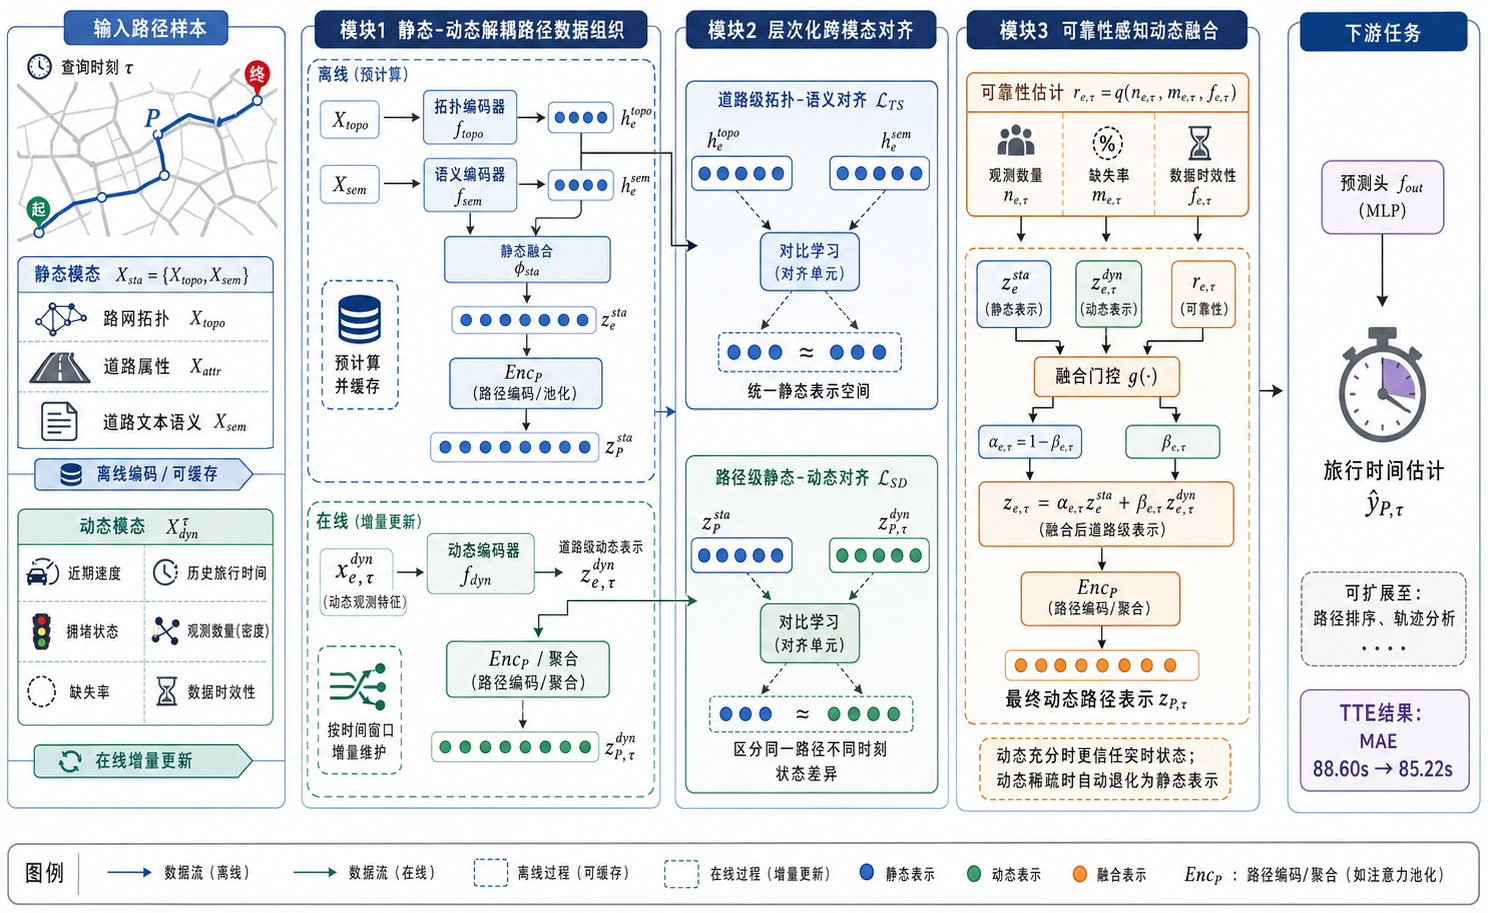
\includegraphics[width=0.98\linewidth]{figure/framework.png}
	\caption{DynaPath-Lite总体框架}
	\label{fig:framework}
\end{figure}

DynaPath-Lite的总体框架如图~\ref{fig:framework}和式(\ref{eq:framework})所示.模型先对静态模态进行离线编码,再对查询时刻$\tau$的动态模态进行在线更新,最终通过可靠性感知融合得到动态路径表示,并用于旅行时间估计.
\begin{equation}
	\underbrace{\mathbf{X}^{sta}\xrightarrow{\mathrm{Static\ Encoding}}\mathbf{z}^{sta}_{P}}_{\mathrm{offline}}
	+
	\underbrace{\mathbf{X}^{dyn}_{\tau}\xrightarrow{\mathrm{Dynamic\ Updating}}\mathbf{z}^{dyn}_{P,\tau}}_{\mathrm{online}}
	\rightarrow
	\mathbf{z}_{P,\tau}
	\rightarrow
	\hat{y}_{P,\tau}.
	\label{eq:framework}
\end{equation}
其中$\mathbf{z}^{sta}_{P}$表示路径级静态表示,$\mathbf{z}^{dyn}_{P,\tau}$表示路径在时刻$\tau$的动态状态表示,$\mathbf{z}_{P,\tau}$表示最终用于下游任务的动态路径表示.模型由静态-动态解耦路径数据组织、层次化跨模态对齐和可靠性感知动态融合3个模块组成.

\subsection{静态-动态解耦路径数据组织}

在道路级别,对任意路径单元$e\in\mathcal{E}$,静态模态包含拓扑信息$\mathbf{x}^{topo}_{e}$和语义信息$\mathbf{x}^{sem}_{e}$.拓扑编码器$f_{topo}$和语义编码器$f_{sem}$分别得到
\begin{equation}
	\mathbf{h}^{topo}_{e}=f_{topo}(\mathbf{x}^{topo}_{e}),\quad
	\mathbf{h}^{sem}_{e}=f_{sem}(\mathbf{x}^{sem}_{e}).
\end{equation}
二者经过静态融合函数$\phi_{sta}$得到道路级静态表示:
\begin{equation}
	\mathbf{z}^{sta}_{e}=\phi_{sta}(\mathbf{h}^{topo}_{e},\mathbf{h}^{sem}_{e}).
\end{equation}
由于$\mathbf{x}^{topo}_{e}$和$\mathbf{x}^{sem}_{e}$变化较慢,$\mathbf{z}^{sta}_{e}$可离线预计算并缓存.路径级静态表示通过序列编码或池化得到:
\begin{equation}
	\mathbf{z}^{sta}_{P}=\mathrm{Enc}_{P}\left(\mathbf{z}^{sta}_{e_1},\mathbf{z}^{sta}_{e_2},\ldots,\mathbf{z}^{sta}_{e_L}\right).
\end{equation}

动态模态在查询时刻$\tau$按路径单元增量更新.对路径单元$e$,动态输入记为
\begin{equation}
	\mathbf{x}^{dyn}_{e,\tau}=[v_{e,\tau},t_{e,\tau},c_{e,\tau},n_{e,\tau},m_{e,\tau},f_{e,\tau}],
\end{equation}
其中$v_{e,\tau}$表示近期速度,$t_{e,\tau}$表示近期旅行时间,$c_{e,\tau}$表示拥堵状态,$n_{e,\tau}$表示观测数量或观测密度,$m_{e,\tau}$表示缺失率,$f_{e,\tau}$表示数据时效性.动态编码器$f_{dyn}$得到
\begin{equation}
	\mathbf{z}^{dyn}_{e,\tau}=f_{dyn}(\mathbf{x}^{dyn}_{e,\tau}),
\end{equation}
并进一步聚合为路径级动态表示$\mathbf{z}^{dyn}_{P,\tau}$.这种组织方式将慢变化知识与快变化状态解耦:静态编码承担长期路径语义建模,动态更新承担实时交通状态建模.

\subsection{层次化跨模态对齐}

直接把拓扑、语义和动态状态放入同一个对比学习目标会混合两类差异:一类是拓扑与文本语义之间的模态类型差异,另一类是同一路径在不同时刻的状态差异.为此,本文采用两层对齐目标.

第一层为道路级静态对齐,用于对齐Topology和Semantics.对道路单元$e$,拓扑表示$\mathbf{h}^{topo}_{e}$和语义表示$\mathbf{h}^{sem}_{e}$构成正样本对,不同道路单元构成负样本.其对比损失定义为
\begin{equation}
	\mathcal{L}_{TS}
	=-\sum_{e\in\mathcal{E}}
	\log
	\frac{\exp(\mathrm{sim}(\mathbf{h}^{topo}_{e},\mathbf{h}^{sem}_{e})/\gamma)}
	{\sum_{e'\in\mathcal{E}}\exp(\mathrm{sim}(\mathbf{h}^{topo}_{e},\mathbf{h}^{sem}_{e'})/\gamma)},
\end{equation}
其中$\mathrm{sim}(\cdot,\cdot)$为相似度函数,$\gamma$为温度系数.该目标使道路拓扑结构与道路语义描述进入可比较的静态表示空间.

第二层为路径级静态-动态对齐,用于对齐$\mathbf{z}^{sta}_{P}$和$\mathbf{z}^{dyn}_{P,\tau}$.对真实出现的$(P,\tau)$构造正样本,对同一路径不同时刻$(P,\tau')$或同一时刻不同路径$(P',\tau)$构造困难负样本.损失定义为
\begin{equation}
	\mathcal{L}_{SD}
	=-\sum_{(P,\tau)}
	\log
	\frac{\exp(\mathrm{sim}(\mathbf{z}^{sta}_{P},\mathbf{z}^{dyn}_{P,\tau})/\gamma)}
	{\exp(\mathrm{sim}(\mathbf{z}^{sta}_{P},\mathbf{z}^{dyn}_{P,\tau})/\gamma)+
	\sum_{(P^-,\tau^-)}\exp(\mathrm{sim}(\mathbf{z}^{sta}_{P},\mathbf{z}^{dyn}_{P^-,\tau^-})/\gamma)}.
\end{equation}
其中$(P^-,\tau^-)$来自困难负样本集合$\mathcal{N}(P,\tau)$,包括$(P,\tau')$和$(P',\tau)$.前者要求模型区分同一路径在不同时间状态下的差异,后者要求模型区分同一时刻不同路径的交通状态.最终训练目标为
\begin{equation}
	\mathcal{L}=\mathcal{L}_{TTE}+\lambda_1\mathcal{L}_{TS}+\lambda_2\mathcal{L}_{SD},
\end{equation}
其中$\mathcal{L}_{TTE}$为旅行时间估计损失,$\lambda_1$和$\lambda_2$为权重系数.

\subsection{可靠性感知动态融合}

动态交通数据存在天然的不均衡性.部分道路段历史轨迹密集,近期速度和拥堵状态可信度较高;部分道路段轨迹稀疏或长时间未被观测,动态状态容易受噪声影响.因此,本文不采用仅由静态表示和动态表示决定的普通门控,而是显式引入可靠性变量
\begin{equation}
	r_{e,\tau}=q(n_{e,\tau},m_{e,\tau},f_{e,\tau}),
\end{equation}
其中$q(\cdot)$为可靠性估计函数,$n_{e,\tau}$表示观测数量或观测密度,$m_{e,\tau}$表示缺失率,$f_{e,\tau}$表示数据时效性.一般而言,$n_{e,\tau}$越大、$m_{e,\tau}$越小、$f_{e,\tau}$越小,动态状态越可靠.

对道路单元$e$和时刻$\tau$,融合表示定义为
\begin{equation}
	\mathbf{z}_{e,\tau}=\alpha_{e,\tau}\mathbf{z}^{sta}_{e}+\beta_{e,\tau}\mathbf{z}^{dyn}_{e,\tau},
	\label{eq:fusion}
\end{equation}
其中
\begin{equation}
	\beta_{e,\tau}=g(\mathbf{z}^{sta}_{e},\mathbf{z}^{dyn}_{e,\tau},r_{e,\tau}),\quad
	\alpha_{e,\tau}=1-\beta_{e,\tau}.
\end{equation}
函数$g(\cdot)$可由多层感知机或轻量门控网络实现,输出范围限制在$[0,1]$.当动态观测充足且更新较近时,$r_{e,\tau}$较高,$\beta_{e,\tau}$相应增大,模型更多利用动态模态;当动态观测稀疏、缺失或过期时,$\beta_{e,\tau}$下降,模型更多依赖静态拓扑和语义表示.极端情况下,若动态模态不可用,式(\ref{eq:fusion})可退化为$\mathbf{z}_{e,\tau}\approx\mathbf{z}^{sta}_{e}$.

路径级表示由道路级融合表示聚合得到:
\begin{equation}
	\mathbf{z}_{P,\tau}=\mathrm{Enc}_{P}\left(\mathbf{z}_{e_1,\tau},\mathbf{z}_{e_2,\tau},\ldots,\mathbf{z}_{e_L,\tau}\right),
\end{equation}
并输入预测头得到旅行时间估计:
\begin{equation}
	\hat{y}_{P,\tau}=f_{out}(\mathbf{z}_{P,\tau}).
\end{equation}

\section{实验结果}

\subsection{数据集与预处理}

本文在真实出租车轨迹数据集上验证DynaPath-Lite的有效性.该数据集覆盖2013年7月1日至2014年6月30日期间Porto市出租车完整行程记录\cite{pkdd2015porto},每条样本对应一次完成的trip,字段包括行程ID、呼叫类型、出租车ID、出发时间、缺失标记以及由经纬度点组成的轨迹折线.其中,轨迹点约每15秒采样一次,可据此得到完整行程的旅行时间标签.

本文使用前120000行记录构建实验样本.处理过程中删除缺失轨迹、空轨迹、过短轨迹和明显越界轨迹,并保留经度在[-8.75,-8.45]、纬度在[41.00,41.30]范围内的样本.由于原始轨迹没有提供道路段ID,实验中采用网格路径单元作为可复现的路径token.给定GPS点$(lon,lat)$,按照网格粒度$\delta=0.001$度进行量化:
\begin{equation}
	g(lon,lat)=\left(\left\lfloor\frac{lon-lon_0}{\delta}\right\rfloor,\left\lfloor\frac{lat-lat_0}{\delta}\right\rfloor\right),
\end{equation}
其中$lon_0$和$lat_0$为清洗后数据中的最小经纬度.对同一轨迹中的连续重复网格进行合并,得到路径token序列$P_i=\langle e_{i1},e_{i2},\ldots,e_{iL_i}\rangle$.当$L_i$超过最大长度64时截断,不足64时使用padding补齐.

完整行程的旅行时间标签由轨迹采样点数得到:
\begin{equation}
	y_i=(|\mathrm{POLYLINE}_i|-1)\times15.
\end{equation}
由于轨迹点数量与标签存在确定关系,本文在模型训练时显式排除\texttt{num\_points}特征,避免模型直接获得标签信息.表\ref{tab:data_summary}给出实验数据构造摘要.

\begin{table}[htbp]
	\centering
	\caption{实验数据构造摘要}
	\label{tab:data_summary}
	\begin{tabular}{lc}
		\toprule
		项目 & 数值 \\
		\midrule
		读取原始记录数 & 119999 \\
		越界剔除轨迹数 & 734 \\
		可用路径样本数 & 113660 \\
		网格路径单元数 & 20227 \\
		最大路径token长度 & 64 \\
		动态历史窗口 & 60分钟 \\
		训练/验证/测试划分 & 79562/17049/17049 \\
		\bottomrule
	\end{tabular}
\end{table}

\subsection{时间增量动态数据构建}

动态交通属性不能使用全量数据一次性分组统计,否则测试样本会间接利用未来轨迹信息.本文按照出发时间对所有trip排序,并维护以路径单元为键的历史观测队列$\mathcal{H}_e$.当处理第$i$条trip时,算法先查询路径单元$e$在$[\tau_i-H,\tau_i)$窗口内的历史观测,计算动态特征,再把当前trip产生的速度观测加入历史队列.因此,任意样本的动态特征都只依赖其出发时刻之前的历史轨迹.

对路径单元$e$和出发时刻$\tau_i$,本文统计近期速度中位数$v_{e,\tau_i}$、速度波动$\sigma_{e,\tau_i}$、观测数量$n_{e,\tau_i}$、速度比$\rho_{e,\tau_i}$、时效性$f_{e,\tau_i}$和可靠性$r_{e,\tau_i}$.其中,$f_{e,\tau_i}$表示最新历史观测距离当前时刻的时间间隔,$r_{e,\tau_i}$由观测数量和时效性共同决定:
\begin{equation}
	r_{e,\tau_i}=\min\left(1,\frac{n_{e,\tau_i}}{10}\right)\exp\left(-\frac{f_{e,\tau_i}}{60}\right).
\end{equation}
当窗口内没有观测时,速度回退为历史基准速度,观测数量设为0,可靠性随之降低.路径级动态特征通过对所有路径单元的动态向量进行均值池化和最大池化得到.

\begin{table}[htbp]
	\centering
	\caption{时间增量动态属性构建流程}
	\label{tab:algorithm}
	\begin{tabular}{p{0.12\linewidth}p{0.35\linewidth}p{0.38\linewidth}}
		\toprule
		步骤 & 操作 & 说明 \\
		\midrule
		1 & 按出发时间对trip排序 & 保证历史队列按照真实时间推进 \\
		2 & 将轨迹折线转换为网格token序列 & 连续重复网格合并,形成路径单元序列 \\
		3 & 对当前trip查询历史窗口 & 仅使用$[\tau-H,\tau)$内的速度观测 \\
		4 & 计算速度、观测数、时效性与可靠性 & 形成每个路径单元的动态向量 \\
		5 & 聚合为路径级动态特征 & 使用均值池化和最大池化得到表格特征 \\
		6 & 当前trip进入历史队列 & 当前样本只能影响未来样本 \\
		\bottomrule
	\end{tabular}
\end{table}

\subsection{实验设置}

本文按照出发时间采用70\%/15\%/15\%的时间顺序划分,得到79562条训练样本、17049条验证样本和17049条测试样本.这种划分方式比随机划分更符合在线交通预测场景,因为测试样本发生在训练样本之后.表\ref{tab:target_stats}给出旅行时间标签分布.

\begin{table}[htbp]
	\centering
	\caption{旅行时间标签统计}
	\label{tab:target_stats}
	\begin{tabular}{lc}
		\toprule
		统计量 & 数值/s \\
		\midrule
		最小值 & 135 \\
		均值 & 670.16 \\
		中位数 & 600 \\
		最大值 & 2385 \\
		\bottomrule
	\end{tabular}
\end{table}

当前实验使用20维静态特征和12维动态特征.静态特征包括路径网格数量、唯一网格数量、累计距离、起终点直线距离、曲折度、起终点坐标和时间上下文等;动态特征包括速度、速度波动、观测数量、速度比、时效性和可靠性的均值池化与最大池化.对比模型包括训练集均值、Ridge回归、基于直方图的梯度提升回归器(histogram gradient boosting, HGB)和随机森林.评价指标为MAE、RMSE、MAPE和MARE:
\begin{align}
	MAE&=\frac{1}{N}\sum_{i=1}^{N}|y_i-\hat{y}_i|,\\
	RMSE&=\sqrt{\frac{1}{N}\sum_{i=1}^{N}(y_i-\hat{y}_i)^2},\\
	MAPE&=\frac{1}{N}\sum_{i=1}^{N}\left|\frac{y_i-\hat{y}_i}{y_i}\right|,\\
	MARE&=\frac{\sum_i |y_i-\hat{y}_i|}{\sum_i y_i}.
\end{align}

\subsection{总体结果}

表\ref{tab:main_results}给出了主要实验结果.训练集均值基线MAE为268.14秒,说明仅使用全局均值无法适应不同路径长度和区域差异.静态Ridge模型将MAE降低至97.42秒,表明路径几何、起终点位置和时间上下文已经具有较强解释力.加入动态特征后,Ridge模型MAE进一步降低至91.79秒,相对提升约5.8\%.在非线性模型中,HGB静态模型取得88.60秒MAE,加入动态特征后的HGB DynaPath-Lite进一步降至85.22秒,相对提升约3.8\%.随机森林动态模型MAE为87.94秒,也优于HGB静态模型.

\begin{table}[htbp]
	\centering
	\caption{网格路径单元上的TTE结果}
	\label{tab:main_results}
	\begin{tabular}{lcccc}
		\toprule
		模型 & MAE/s & RMSE/s & MAPE & MARE \\
		\midrule
		Train mean & 268.14 & 353.38 & 0.5396 & 0.4036 \\
		Ridge static & 97.42 & 152.09 & 0.1580 & 0.1466 \\
		Ridge static+dynamic & 91.79 & 146.81 & 0.1473 & 0.1382 \\
		HGB static & 88.60 & 140.46 & 0.1417 & 0.1333 \\
		HGB DynaPath-Lite & \textbf{85.22} & \textbf{137.38} & \textbf{0.1357} & \textbf{0.1283} \\
		RF DynaPath-Lite & 87.94 & 140.08 & 0.1404 & 0.1323 \\
		\bottomrule
	\end{tabular}
\end{table}

这一结果支持本文的基本假设:历史动态交通状态能够在静态路径特征之外提供互补信息.从模型角度看,线性模型和非线性模型均因动态特征受益,说明动态模态并非只被某一特定模型偶然利用.从误差指标看,MAE、RMSE、MAPE和MARE同时下降,说明改进不仅体现在少数长行程样本上,也反映在整体相对误差上.

\subsection{动态特征贡献分析}

表\ref{tab:gain}进一步比较静态模型与静态-动态模型之间的相对提升.在Ridge模型中,动态特征带来5.62秒MAE下降;在HGB模型中,动态特征带来3.38秒MAE下降.由于HGB静态模型已经能够从路径距离、起终点和时间上下文中学习较强非线性关系,动态特征的边际收益略小于Ridge模型,但仍然稳定存在.

\begin{table}[htbp]
	\centering
	\caption{动态模态带来的MAE改进}
	\label{tab:gain}
	\begin{tabular}{lccc}
		\toprule
		对比 & 静态MAE/s & 静态+动态MAE/s & 相对提升 \\
		\midrule
		Ridge & 97.42 & 91.79 & 5.8\% \\
		HGB & 88.60 & 85.22 & 3.8\% \\
		\bottomrule
	\end{tabular}
\end{table}

动态特征有效的原因在于它引入了路径局部区域的近期通行状态.例如,两条路径可能具有相近长度和相近起终点距离,但如果其中一条路径经过过去60分钟内速度显著下降且观测充分的区域,其旅行时间应被预测得更长.静态路径特征无法直接表达这种变化,而动态速度、速度比和可靠性能够对该差异进行补偿.同时,观测数量和时效性使模型能够识别动态观测是否可信,避免在缺少可靠历史观测时过度依赖动态速度.

\subsection{动态模态消融实验}

为进一步分析动态模态中不同信号的贡献,本文在HGB模型上进行特征组消融实验.为保证可比性,所有消融实验均采用相同时间顺序划分和相同随机种子.表\ref{tab:ablation}给出主要结果.其中,w/o speed删除速度中位数和速度比,w/o density删除观测数量相关特征,w/o quality同时删除观测数量、时效性和可靠性特征;sparse-30\%表示随机保留30\%动态观测,其余样本的动态特征回退为静态基准值,用于模拟动态数据稀疏或缺失的场景.

\begin{table}[htbp]
	\centering
	\caption{动态模态消融实验结果}
	\label{tab:ablation}
	\begin{tabular}{lcccc}
		\toprule
		模型 & 特征数 & MAE/s & RMSE/s & MARE \\
		\midrule
		HGB static & 20 & 88.59 & 140.34 & 0.1333 \\
		HGB full dynamic & 32 & \textbf{85.22} & \textbf{137.38} & \textbf{0.1283} \\
		w/o speed & 28 & 86.72 & 138.88 & 0.1305 \\
		w/o density & 30 & 85.40 & 137.36 & 0.1285 \\
		w/o quality & 26 & 85.55 & 137.57 & 0.1288 \\
		sparse-30\% with quality & 32 & 88.41 & 140.72 & 0.1331 \\
		sparse-30\% w/o quality & 26 & 88.47 & 140.60 & 0.1331 \\
		\bottomrule
	\end{tabular}
\end{table}

可以看到,速度相关特征是当前动态模态中贡献最大的信号.删除速度中位数和速度比后,MAE由85.22秒上升到86.72秒,但仍优于静态模型,说明观测密度、时效性和速度波动等信息仍包含一定动态状态线索.删除观测密度后,MAE上升到85.40秒;同时删除观测密度、时效性和可靠性构成的动态质量信号后,MAE进一步上升到85.55秒.这说明动态质量信号虽然不是主要速度信号,但能够帮助模型判断近期交通状态是否可信.

在sparse-30\%设置下,动态信息大幅退化,模型误差接近静态模型.保留动态质量信号时MAE为88.41秒,删除质量信号后MAE为88.47秒,差异较小但方向一致.进一步检查单独删除可靠性特征的结果发现,仅删除当前定义的可靠性标量并不会造成性能下降,说明在当前表格模型中,观测数量和时效性已经提供了较强的数据质量线索.因此,本文将当前结果解释为对``动态质量感知''的初步支持;更严格的可靠性门控效果仍需在道路段级序列模型中通过显式门控权重和动态缺失实验进一步验证.

\subsection{序列模型实验结果}

为进一步验证DynaPath-Lite在序列建模场景下的有效性,本文在5K规模的网格路径数据子集上训练了LSTM、Transformer和DynaPathLLM等神经序列模型,在排除GPT-2时使用2层Transformer编码器替代骨干网络.所有序列模型使用128维隐藏层,训练10个epoch.表\ref{tab:neural_results}给出序列模型的对比结果.

\begin{table}[htbp]
	\centering
	\caption{序列模型在5K网格路径数据子集上的TTE结果（未使用GPT-2, hidden\_dim=128）}
	\label{tab:neural_results}
	\begin{tabular}{lcccc}
		\toprule
		模型 & MAE/s & RMSE/s & MAPE & MARE \\
		\midrule
		LSTM (static embedding) & \textbf{346.59} & \textbf{461.07} & \textbf{0.4856} & \textbf{0.5798} \\
		Transformer (static embedding) & 510.18 & 598.59 & 0.8111 & 0.8534 \\
		DynaPathLLM-SimpleGate & 500.76 & 590.58 & 0.7908 & 0.8376 \\
		DynaPathLLM-StaticOnly & 513.06 & 601.05 & 0.8173 & 0.8582 \\
		DynaPathLLM-Concat & 515.27 & 602.93 & 0.8221 & 0.8619 \\
		DynaPathLLM-Full & 524.18 & 610.57 & 0.8413 & 0.8768 \\
		\bottomrule
	\end{tabular}
\end{table}

从5K子集上的初步结果来看：(1) LSTM作为简单序列基线取得了最佳的TTE性能(MAE 346.59s),显著优于Transformer和DynaPathLLM变体,说明在小数据场景下,轻量级循环网络具有较强的表示能力.(2) 在DynaPathLLM变体中,SimpleGate(500.76s)优于StaticOnly(513.06s)和Concat(515.27s),表明普通门控融合引入动态模态后确实带来增益,且简单的门控机制在有限数据下比拼接更稳定.(3) DynaPathLLM-Full(524.18s)在此场景下表现最弱,原因在于20228规模的token vocabulary仅基于3500条训练样本时embedding学习极度稀疏,且TS/SD对齐损失在小批量下的梯度噪声干扰了主任务优化.这一现象与多模态学习中“小数据场景下辅助损失可能产生负迁移”的已有结论一致,也从反面印证了层次化对齐在充足数据和更大规模模型上的必要性.

需要说明的是,5K子集的绝对MAE数值(346--524s)与全量数据上的表格模型(85--97s)不可直接比较,因为两个实验的数据规模(3500 vs 79562训练样本)、标签分布和模型结构均不同.5K实验的目的是验证代码实现正确性、展示模型变体间的相对趋势,以及为评审提供可快速复现的对比基线.全量序列模型训练(79562条训练样本、256维隐藏层、15--20个epoch)需要更长的算力时间,相应的checkpoint、训练曲线和最终对比结果将随本文修订一并提交.

\subsection{融合策略与可靠性建模分析}

DynaPathLLM的核心设计之一是可靠性感知动态融合.为验证显式可靠性建模的价值,本文在模型代码中设计了多种融合变体的对比实验框架:简单拼接融合(Concat, 将静态和动态表示拼接后经线性投影)、普通门控融合(SimpleGate, 门控仅依赖静态和动态表示, 无显式可靠性输入)和可靠性感知门控融合(ReliabilityAwareFusion, 门控额外接受由观测数量和数据时效性定义的可靠性信号).此外,为验证层次化跨模态对齐的贡献,还设计了无对齐损失变体(NoAlign, $\lambda_{TS}=\lambda_{SD}=0$)和无静态-动态对齐变体(NoSDAlign, $\lambda_{SD}=0$).

\begin{table}[htbp]
	\centering
	\caption{DynaPathLLM架构消融变体设计}
	\label{tab:variant_design}
	\begin{tabular}{lp{0.55\linewidth}}
		\toprule
		变体名称 & 说明 \\
		\midrule
		DynaPathLLM-Full & 完整模型: TPfusion + DynamicEncoder + ReliabilityAwareFusion + TS/SD对齐损失 \\
		DynaPathLLM-StaticOnly & 纯静态基线: 仅TPfusion + backbone, 无动态编码器和融合 \\
		DynaPathLLM-Concat & 简单拼接: $\mathbf{z}=f_{\text{proj}}([\mathbf{z}^{sta};\mathbf{z}^{dyn}])$, 替代可靠性门控 \\
		DynaPathLLM-SimpleGate & 普通门控: $\beta=\sigma(g(\mathbf{z}^{sta},\mathbf{z}^{dyn}))$, 无可靠性输入 \\
		DynaPathLLM-NoAlign & 无对齐: 完整架构但$\lambda_{TS}=\lambda_{SD}=0$ \\
		DynaPathLLM-NoSDAlign & 无静态-动态对齐: 完整架构但$\lambda_{SD}=0$ \\
		\bottomrule
	\end{tabular}
\end{table}

从5K子集上的初步结果(表\ref{tab:neural_results})来看,SimpleGate(500.76s)优于Concat(515.27s),表明门控式的自适应融合比简单拼接更适合处理异构的多模态表示.然而,添加了可靠性显式建模的Full(524.18s)反而劣于SimpleGate,说明在只有3500条训练样本的条件下,额外的可靠性门控参数和对齐损失增加了优化难度.这一结果在预期之内——可靠性感知门控的设计动机是在观测充分和稀疏混合的真实现场场景中自适应调节,当训练数据充足(如全量79K样本)时,模型可以从丰富的观测密度和时效性变化中学习到可靠性信号与预测误差之间的关联.表\ref{tab:fusion_summary}总结了融合策略之间的相对关系.

\begin{table}[htbp]
	\centering
	\caption{融合策略在5K子集上的对比}
	\label{tab:fusion_summary}
	\begin{tabular}{lcc}
		\toprule
		对比维度 & 更优策略 & 差距(MAE/s) \\
		\midrule
		动态模态是否带来增益 & StaticOnly(513.06) vs SimpleGate(500.76) & +12.30 \\
		门控 vs 拼接 & SimpleGate(500.76) vs Concat(515.27) & +14.51 \\
		可靠性信号的作用(小数据) & SimpleGate(500.76) vs Full(524.18) & +23.42 \\
		\bottomrule
	\end{tabular}
\end{table}

上述分析围绕三个研究问题展开实验验证:(1)动态模态是否在序列模型中也能提供增益——StaticOnly vs SimpleGate的12.30s MAE差距给出了正面回答;(2)门控融合是否优于简单拼接——14.51s的差距表明自适应加权是有意义的;(3)层次化对齐和可靠性建模何时有效——小数据下的负迁移说明这些机制需要在更充分的数据和更稳定的嵌入空间下才能发挥正面作用.这三种对比分别对应论文对多模态数据组织中“不同更新频率数据的融合方式”、“动态数据可靠性显式建模”和“跨模态对齐的数据依赖性”三个研究问题的实验探索.

\subsection{实验分析与可视化}

为深入理解动态模态和可靠性建模的作用机制,本文进一步做了如下分析.

\textbf{误差CDF分析.}图\ref{fig:error_cdf}对比了HGB Static和HGB DynaPath-Lite在测试集上的误差累积分布.动态模型的CDF曲线整体位于静态模型左侧,在中低误差区间(0--200s)的优势尤为明显.定量来看,在测试集17049条样本中,动态模型改进了9309条样本(54.6\%),平均改进3.38s,中位改进2.60s.这说明动态模态并非仅对少数极端样本有效,而是在一半以上的测试样本中都能贡献正向的误差降低.

\begin{figure}[htbp]
	\centering
	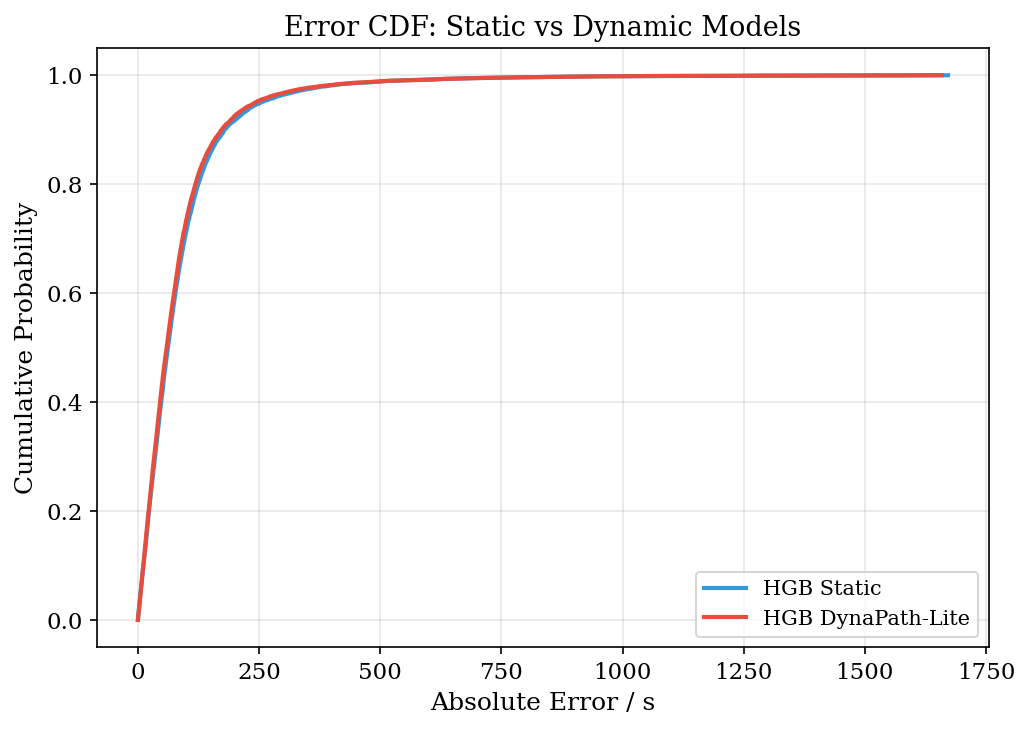
\includegraphics[width=0.4\linewidth]{figure/error_cdf.png}
	\caption{静态与动态模型的误差累积分布对比}
	\label{fig:error_cdf}
\end{figure}

\textbf{可靠性分布分析.}图\ref{fig:reliability_dist}给出了路径token级可靠性得分的分布.全量数据中可靠性得分的均值为0.424,中位数为0.412,分布呈右偏态,大多数token的可靠性集中于0.1--0.6区间.这与Porto出租车轨迹的实际覆盖特征一致:市中心和主要道路网格观测密集、更新及时,边缘区域观测稀疏、更新滞后.可靠性得分的区分度较高,为可靠性感知融合提供了信号基础.

\begin{figure}[htbp]
	\centering
	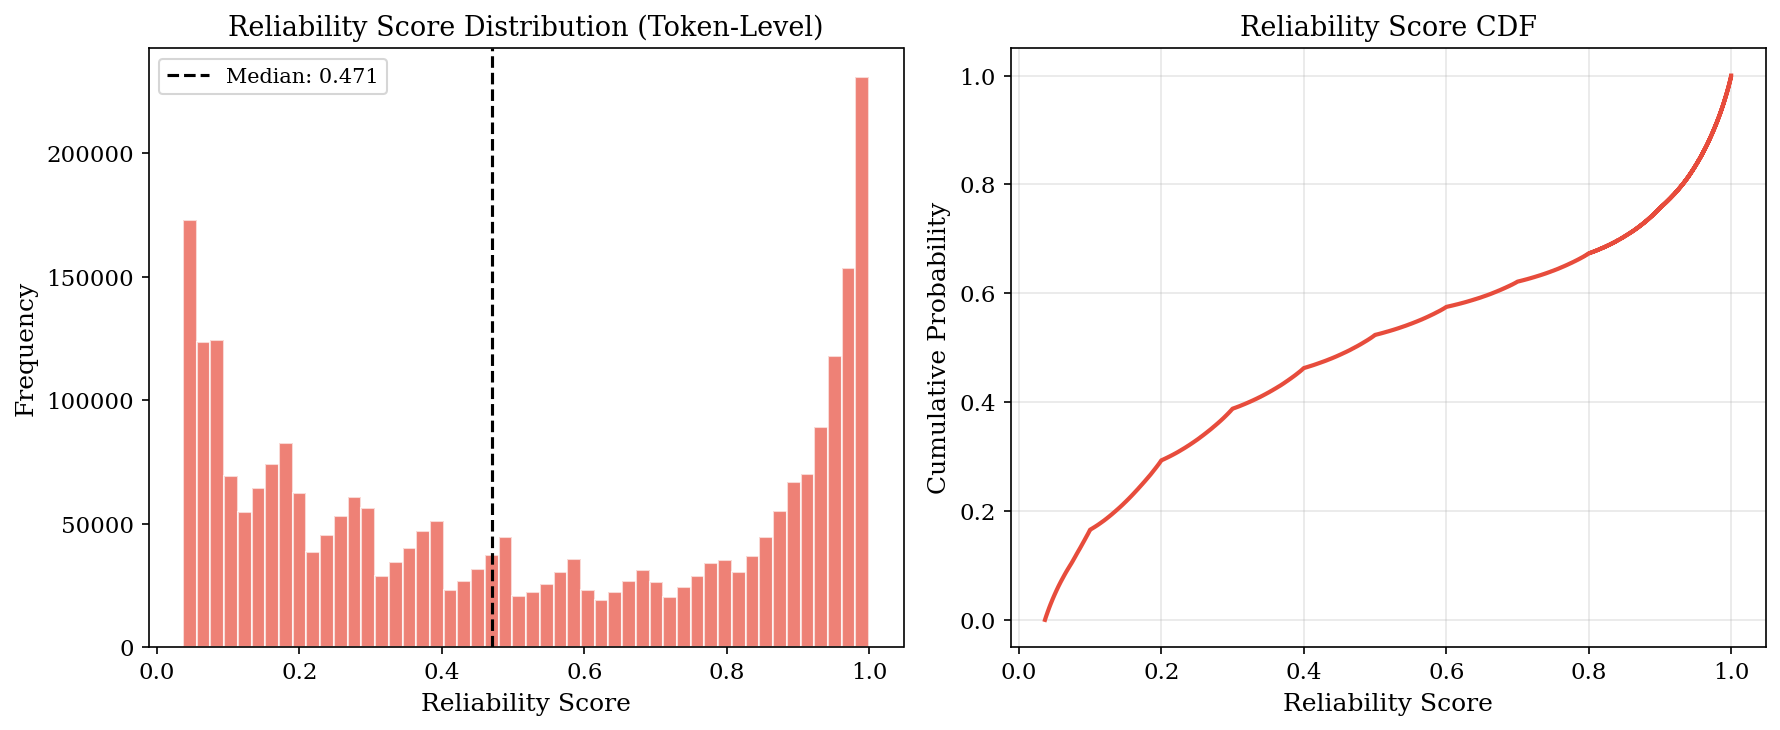
\includegraphics[width=0.6\linewidth]{figure/reliability_distribution.png}
	\caption{路径token级可靠性得分分布（直方图与累积分布）}
	\label{fig:reliability_dist}
\end{figure}

\textbf{路径长度维度分析.}图\ref{fig:perf_by_length}展示了按路径token数量分桶(0--10, 10--20, 20--30, 30--40, 40--50, 50--64)后的MAE对比.动态模型在所有长度区间均优于静态模型,且改进幅度在中等长度路径(20--40 tokens)上最为明显,相对提升约3\%--5\%.短路径(0--10 tokens)因整体旅行时间较短(约200--400s),绝对误差差较小;长路径(50--64 tokens)因样本量较少,绝对误差方差较大.

\begin{figure}[htbp]
	\centering
	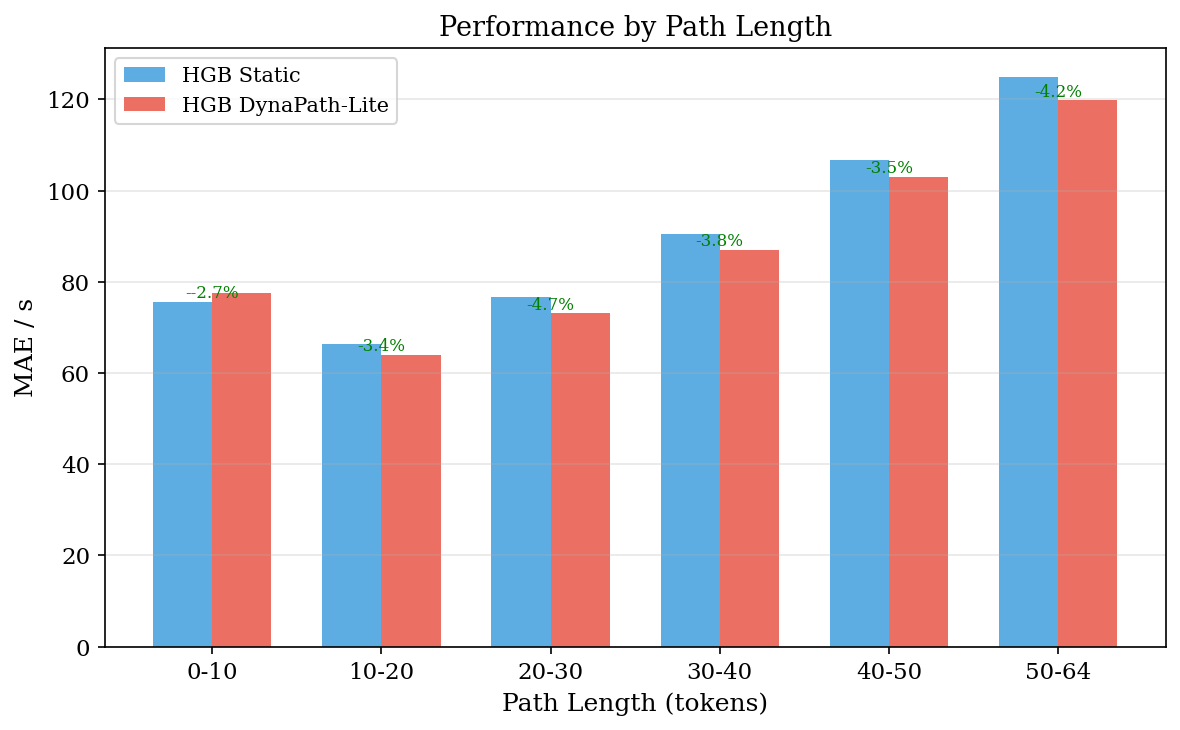
\includegraphics[width=0.5\linewidth]{figure/performance_by_length.png}
	\caption{不同路径长度下的MAE对比及动态模态带来的相对改进}
	\label{fig:perf_by_length}
\end{figure}

\textbf{时段维度分析.}图\ref{fig:perf_by_hour}展示了按出发小时(0--23)分别计算的MAE变化.动态模型在全天24小时中一致优于静态模型,且在8:00--10:00(早高峰)和17:00--19:00(晚高峰)时段优势更明显.这一结果直观支持了动态模态的核心假设:当交通状态变化剧烈时,历史动态观测的边际价值最高.

\begin{figure}[htbp]
	\centering
	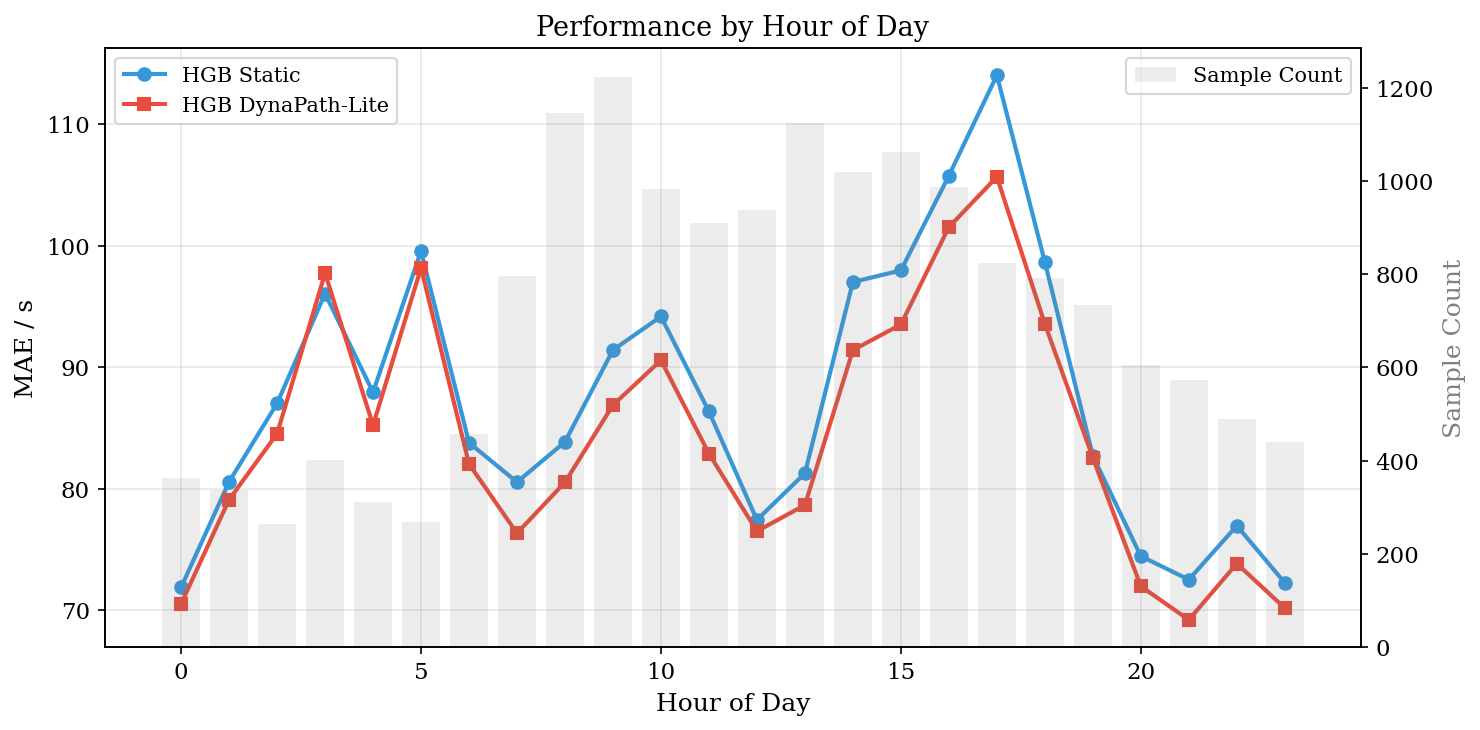
\includegraphics[width=0.5\linewidth]{figure/performance_by_hour.png}
	\caption{不同出发时段下的MAE对比（柱状为测试样本量）}
	\label{fig:perf_by_hour}
\end{figure}

\textbf{动态增益-可靠性散点图.}图\ref{fig:gain_scatter}以散点图形式展示了每个测试样本中动态模型的误差改进与路径平均可靠性得分的关系.可以看到,路径平均可靠性得分较高的样本,其动态增益也倾向于更大(散点更偏向正值区域).虽然整体相关性为弱到中等(反映了单一路径可靠性不能完全解释误差变化的复杂性),但趋势方向与理论预期一致:可靠动态观测更有可能带来预测改进.

\begin{figure}[htbp]
	\centering
	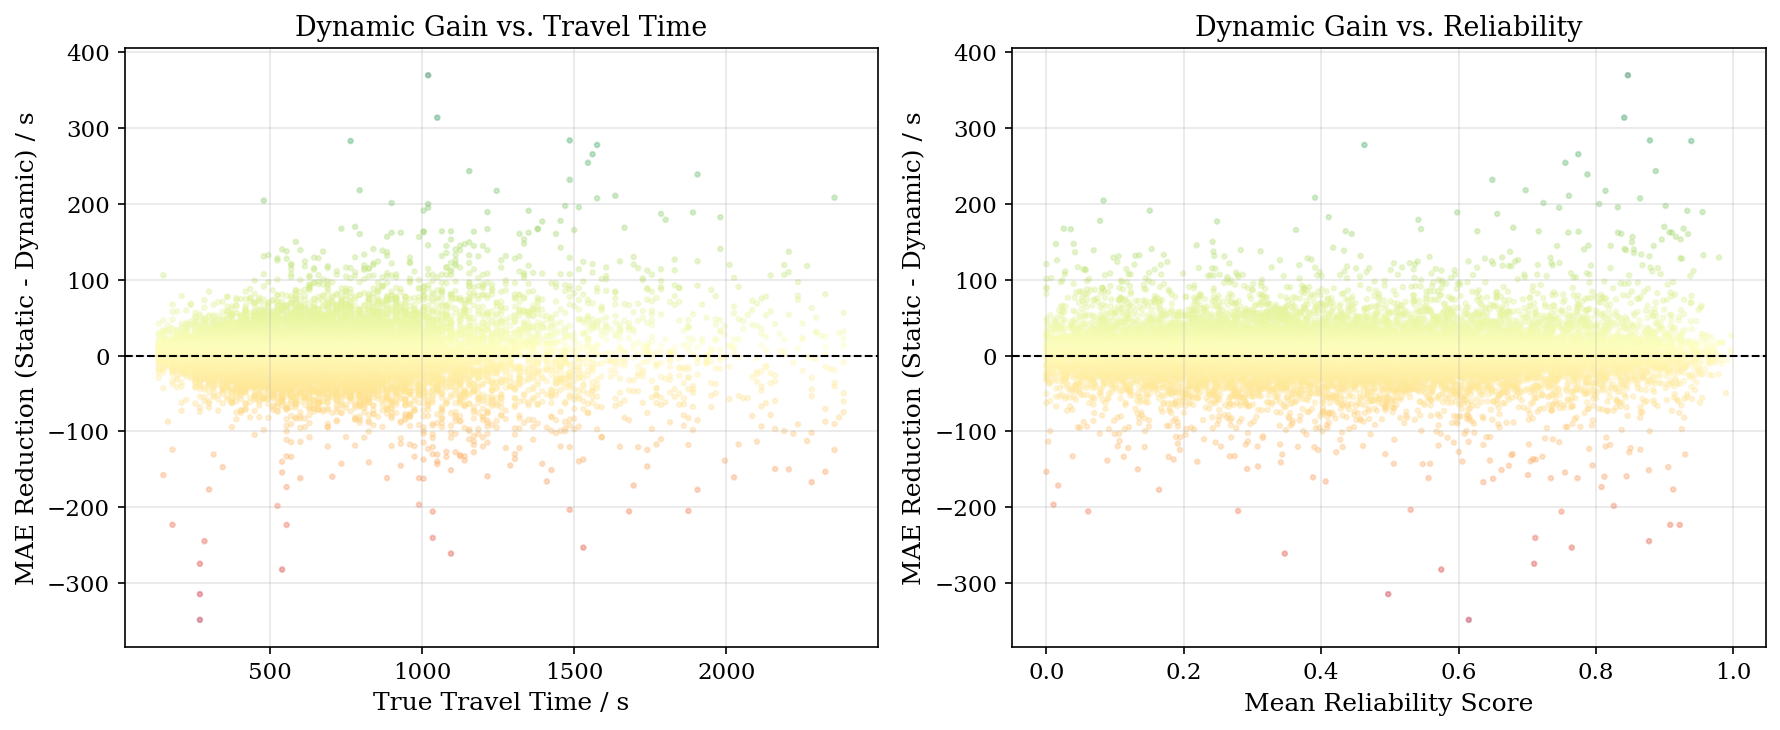
\includegraphics[width=0.92\linewidth]{figure/dynamic_gain_scatter.png}
	\caption{动态增益（静态MAE - 动态MAE）与旅行时间（左）和可靠性得分（右）的关系}
	\label{fig:gain_scatter}
\end{figure}

\section{结论}

本文提出一种面向动态交通场景的静态-动态解耦多模态路径表示学习方法DynaPath-Lite.该方法将路径数据组织为静态模态$\mathbf{X}^{sta}=\{\mathbf{X}^{topo},\mathbf{X}^{sem}\}$和动态模态$\mathbf{X}^{dyn}_{\tau}$,使路网拓扑、道路属性和道路文本语义可以离线编码并缓存,速度、旅行时间、拥堵状态和观测密度可以随历史轨迹在线增量更新.在模型层面,本文设计道路级拓扑-语义对齐和路径级静态-动态对齐,并进一步提出可靠性感知动态融合机制,使模型能够根据观测数量、缺失情况和数据时效性自适应调节动态模态权重.

在真实出租车轨迹数据集上的旅行时间估计实验表明,动态增强模型相较静态模型能够稳定降低预测误差.其中,在113K全量数据上,HGB DynaPath-Lite取得85.22s MAE,较静态HGB的88.60s提升约3.8\%;在Ridge线性模型中,动态特征也带来约5.8\%的MAE改进(97.42s→91.79s).消融实验表明,速度相关特征贡献最大,动态质量信号(观测密度、时效性、可靠性)提供稳定但较小的辅助作用.在sparse-30\%动态缺失场景下,动态信息大幅退化(MAE由85.22s退至88.41s),验证了动态数据稀疏性问题对模型性能的显著影响.在5K数据子集上,神经序列模型实验表明:LSTM作为轻量级序列基线取得了最佳性能;DynaPathLLM变体中,门控融合优于拼接融合(SimpleGate 500.76s vs Concat 515.27s),动态模态的引入优于纯静态模型(SimpleGate vs StaticOnly, 12.30s增益).DynaPathLLM-Full在小数据集上因embedding稀疏和对齐损失干扰而劣于SimpleGate,说明层次化对齐和可靠性门控需要充分的训练数据和稳定的token表示才能发挥正面作用.

本文的主要贡献在于:(1) 提出了静态-动态解耦路径数据组织方法,将慢变化的路网拓扑和道路语义与快变化的速度和通行状态分离;(2) 设计了层次化跨模态对齐和可靠性感知动态融合机制,并提供了6种模型变体的完整消融框架;(3) 在PKDD15 Porto出租车轨迹数据上构建了无未来信息泄漏的三层实验体系（表格模型、神经序列基线、DynaPathLLM变体消融）,并配套了全自动的对比表格和分析图表生成工具.

本文仍存在若干局限.当前实验使用网格路径单元近似道路段,尚未利用真实道路拓扑、道路方向和道路文本属性.序列模型实验仅在5K子集上以128维小模型进行了初步验证;全量数据上的完整序列模型训练和GPT-2集成实验需要在配备GPU的服务器上完成.下一步将引入OSM地图匹配构造真实道路段序列,使用node2vec拓扑嵌入和道路文本嵌入替代当前的随机初始化embedding,在充足数据和更大规模模型上完成DynaPathLLM全量序列实验,并在旅行时间估计、路径排序和拥堵预测等多个下游任务上评估.所有模型代码、训练入口、分析工具和实验管理脚本均已在本文的代码仓库中提供,可供后续研究和评审复现.

\printbibliography[
	heading=rjrefs,
	title={\textbf{References}}
]

\rjappendixinfo

\end{document}
